\documentclass[dissertation.tex]{subfiles}
\begin{document}

This appendix contains figures that visualize the Kernel Density Estimation
(KDE) discrepancies when using activation function $\tanh$ or ReLu.
\begin{itemize}
  \item{
      $\tanh$:
    }
  \item{
      ReLu:
    }
\end{itemize}

% KDE Training Set
\begin{figure}[ht]
  \centering
  \begin{subfigure}[t]{0.32\textwidth}
    \centering
    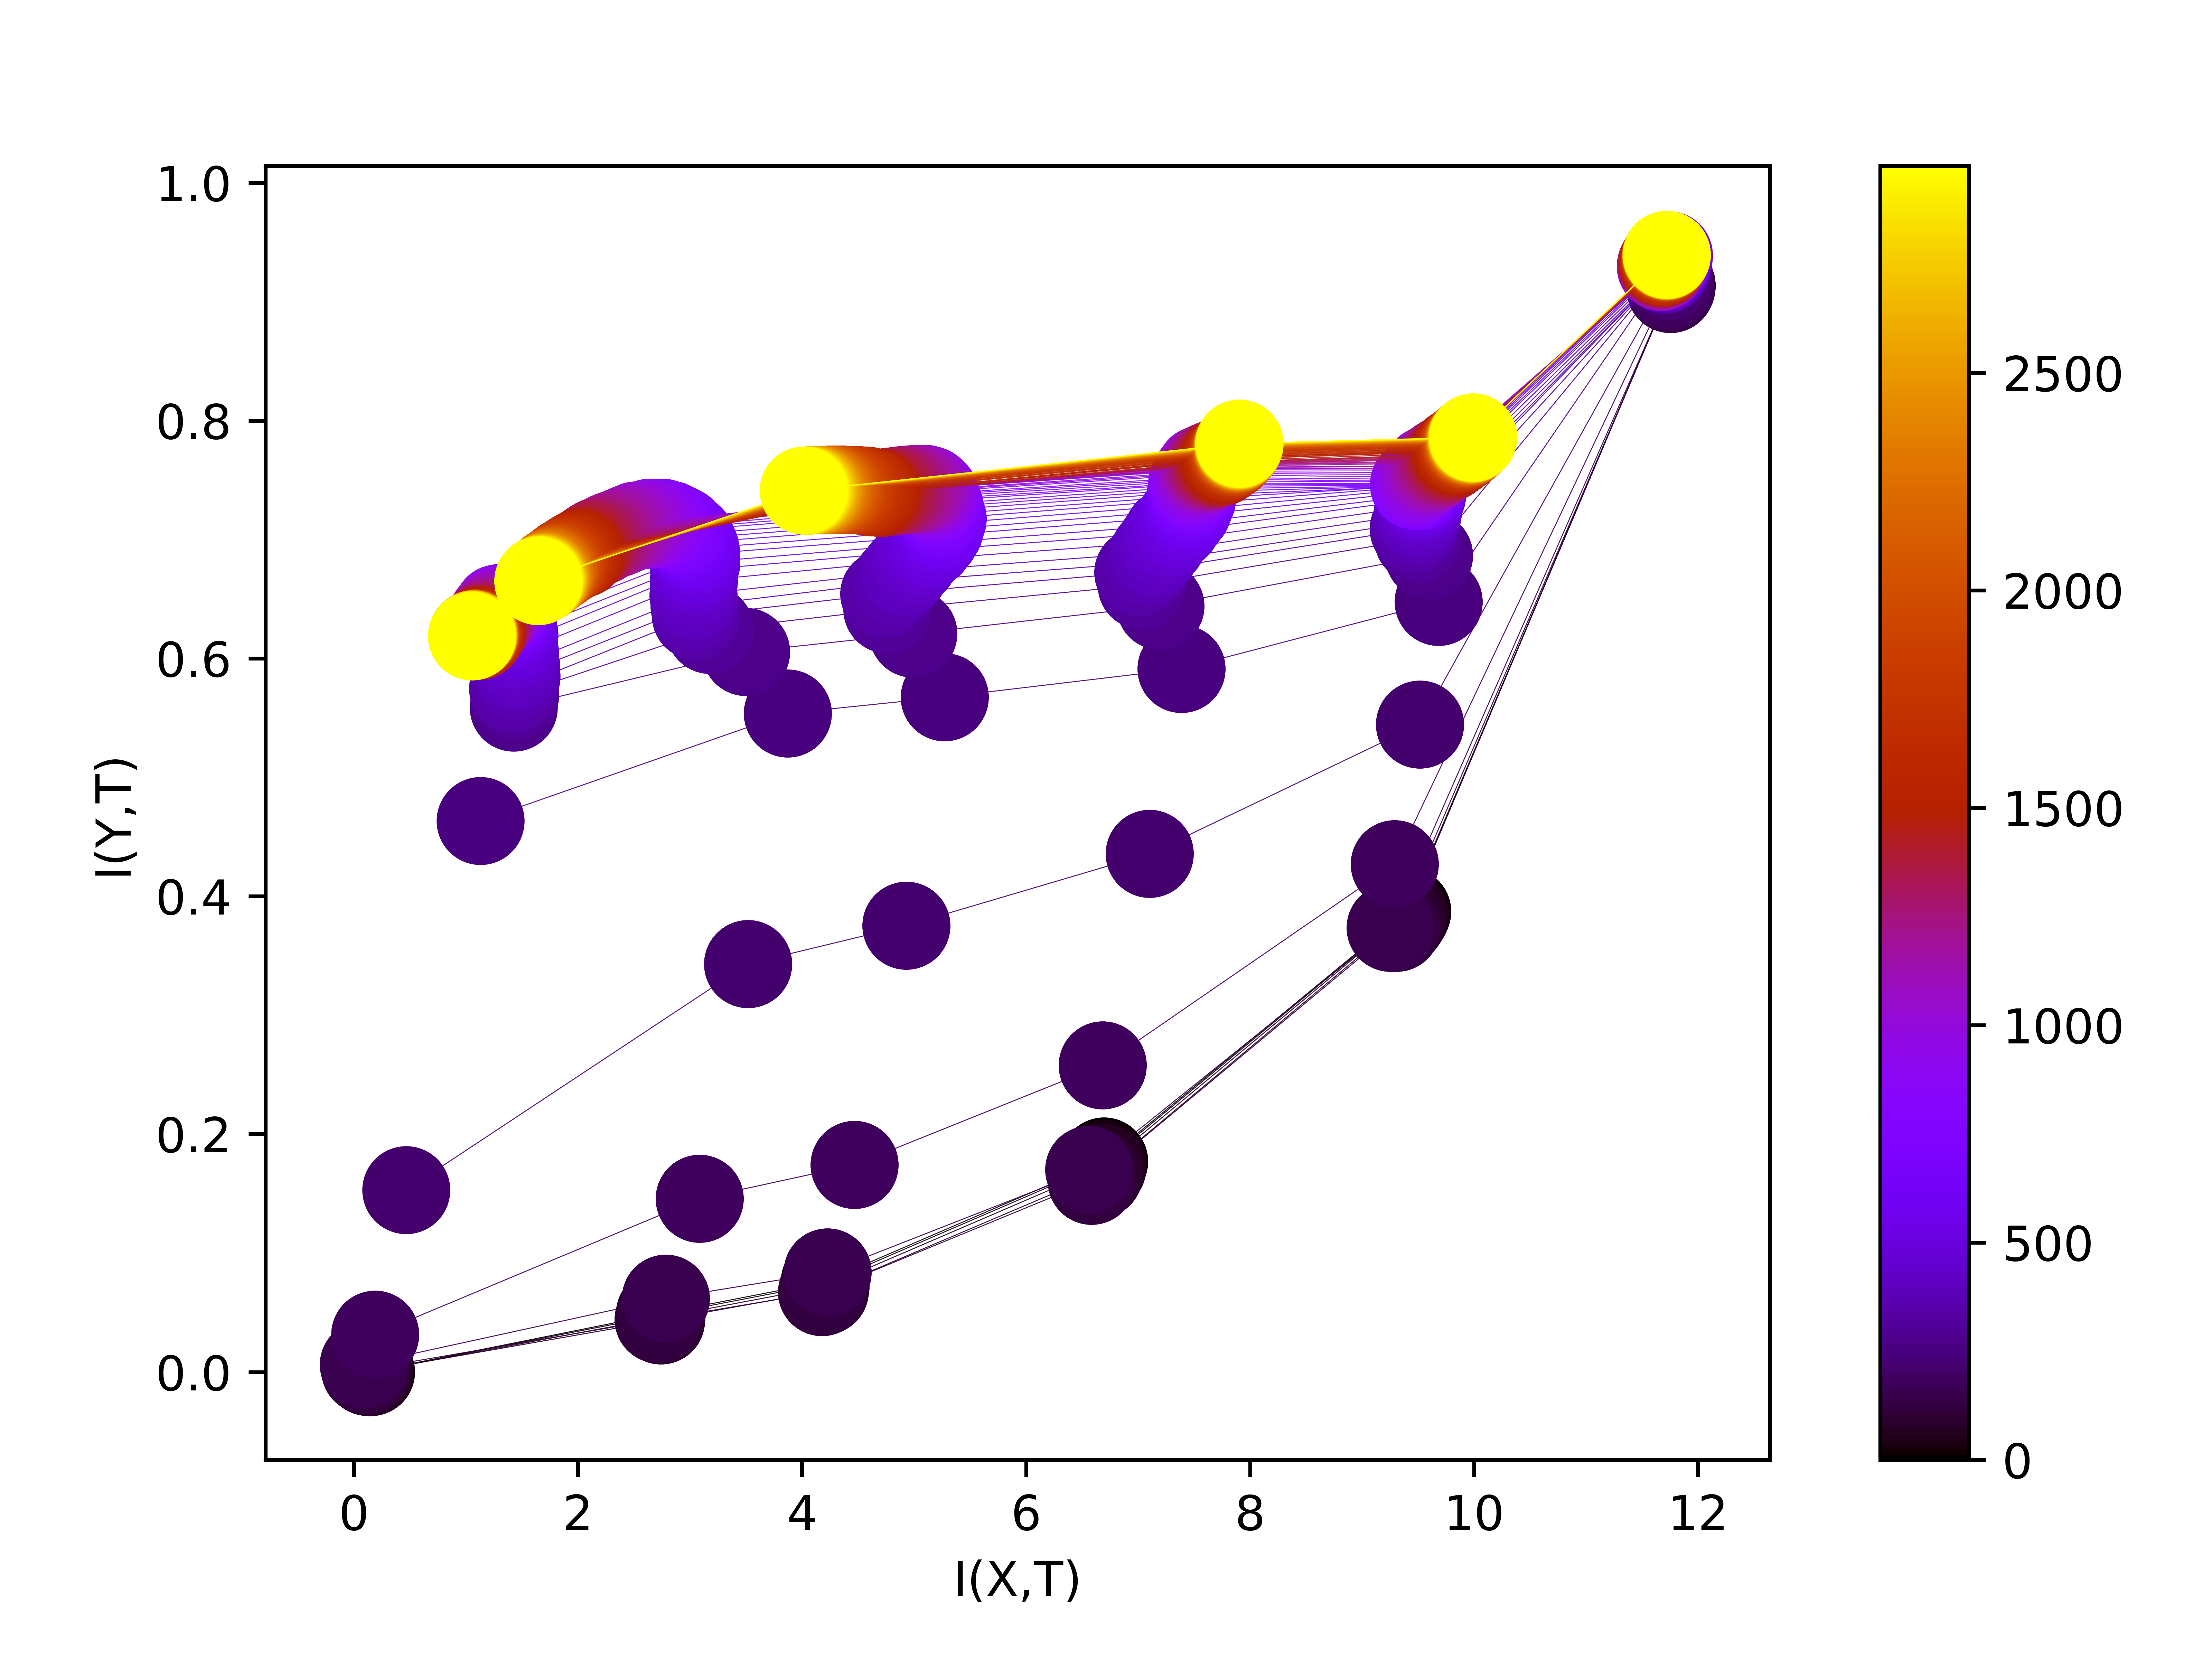
\includegraphics[width=\textwidth]{figs/eval/trainingSize/KDE20.png}
    \caption{
      Training size - 20\%
    }
    \label{figKDETS20}
  \end{subfigure}
  \begin{subfigure}[t]{0.32\textwidth}
    \centering
    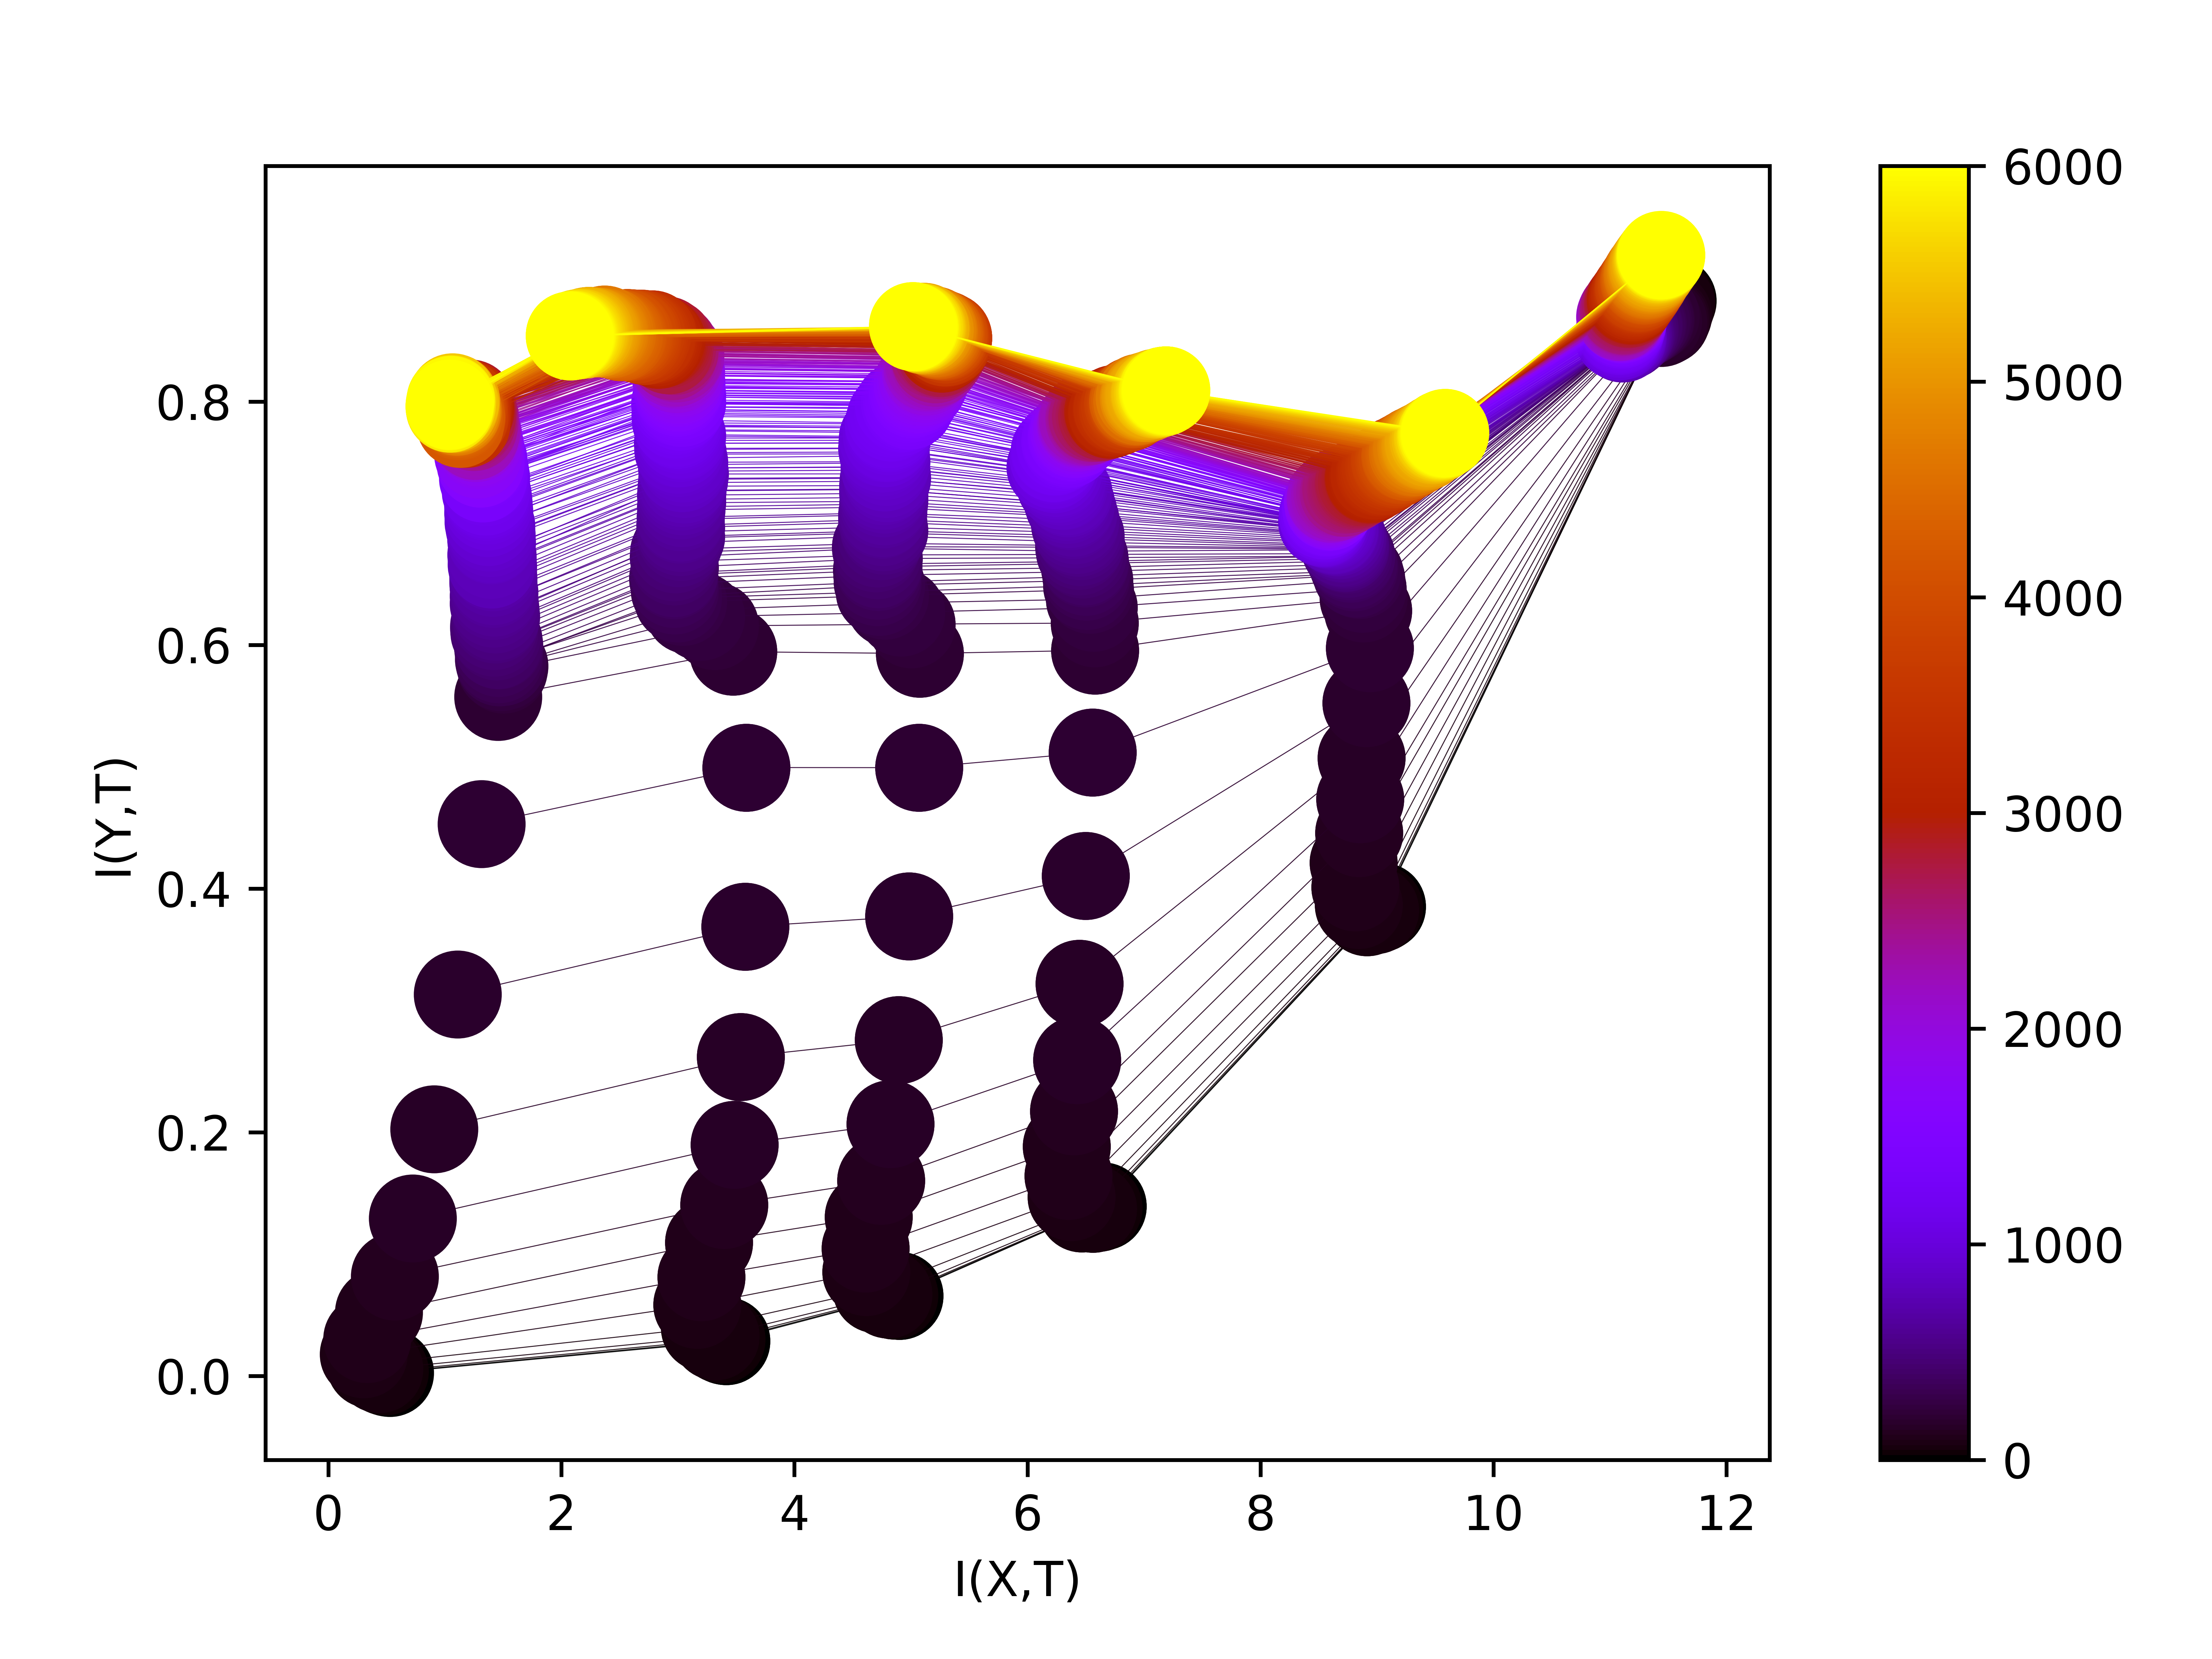
\includegraphics[width=\textwidth]{figs/eval/trainingSize/KDE40.png}
    \caption{
      Training size - 40\%
    }
    \label{figKDETS40}
  \end{subfigure}
  \begin{subfigure}[t]{0.32\textwidth}
    \centering
    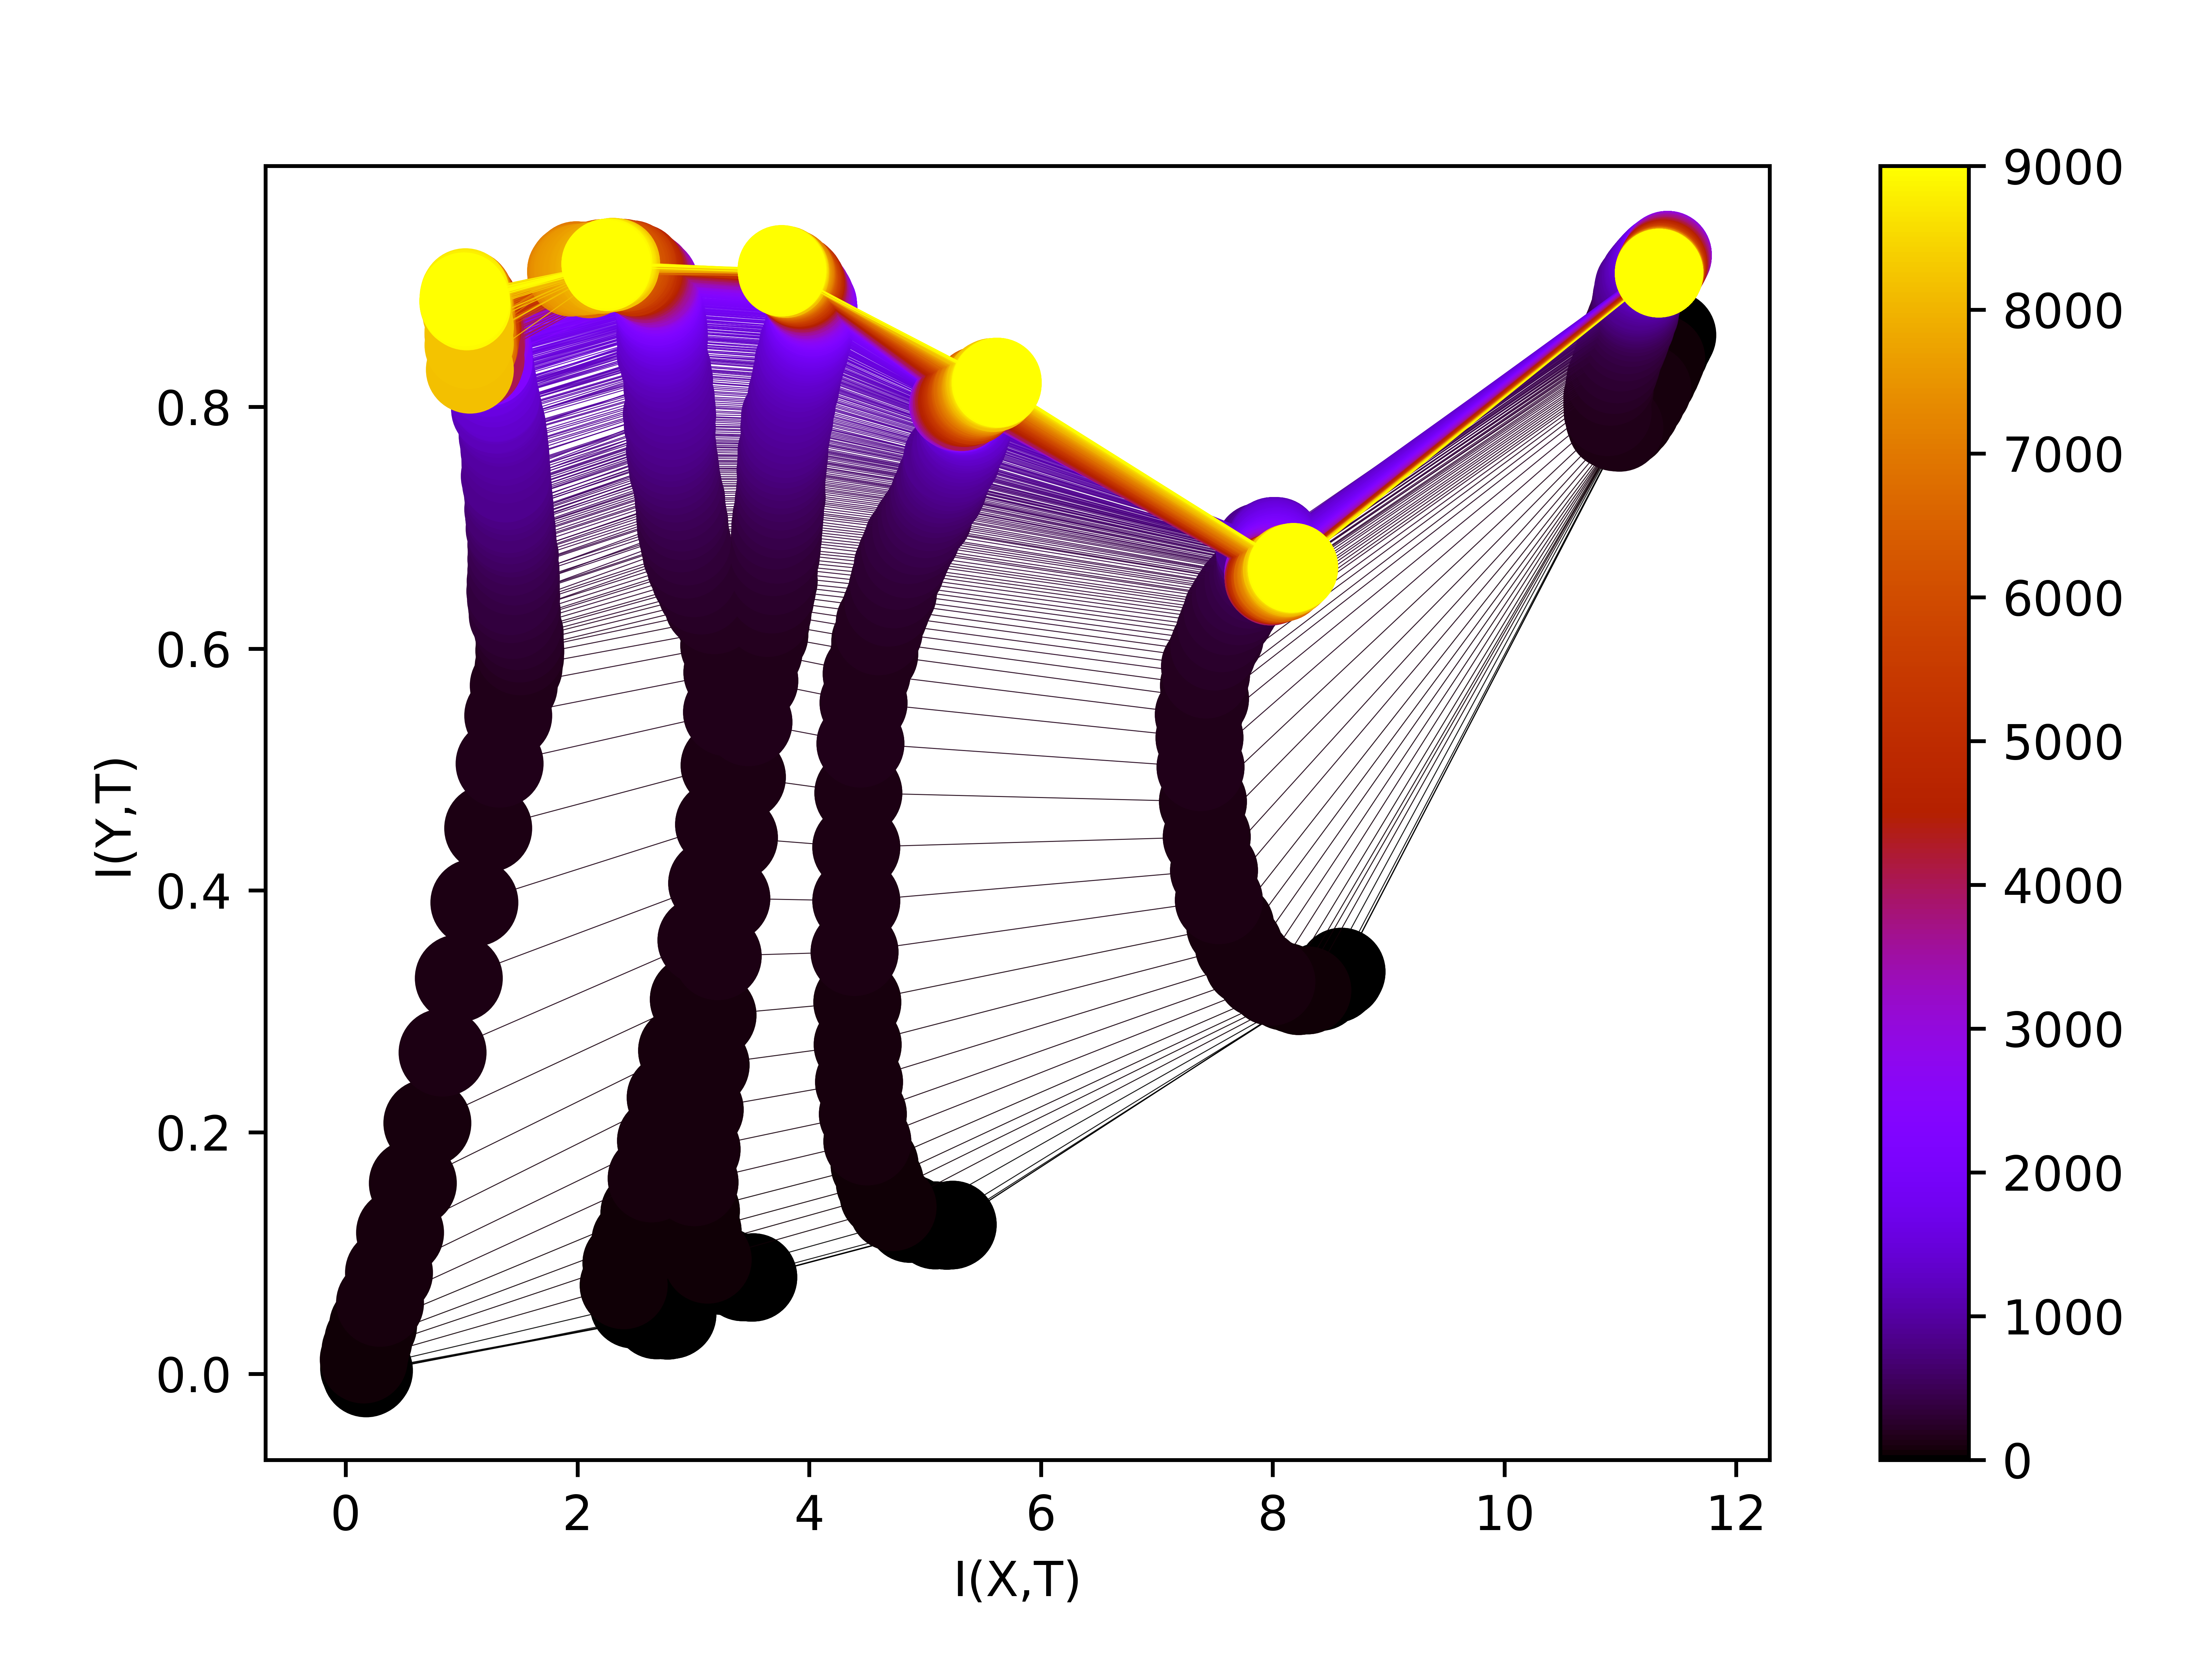
\includegraphics[width=\textwidth]{figs/eval/trainingSize/KDE70.png}
    \caption{
      Training size - 70\%
    }
    \label{figKDETS70}
  \end{subfigure}
  \caption{
      $\tanh$: Demonstrating KDE for different training sizes.  Tweaking training
      size for Tishby's KDE MIE. Hyperparameters: Dataset - Tishby's, activation
      function - $\tanh$, batch size - 512, network shape 12,10,8,6,4,2.
    }
  \label{figKDETS}
\end{figure}

\begin{figure}[ht]
  \centering
  \begin{subfigure}[t]{0.32\textwidth}
    \centering
    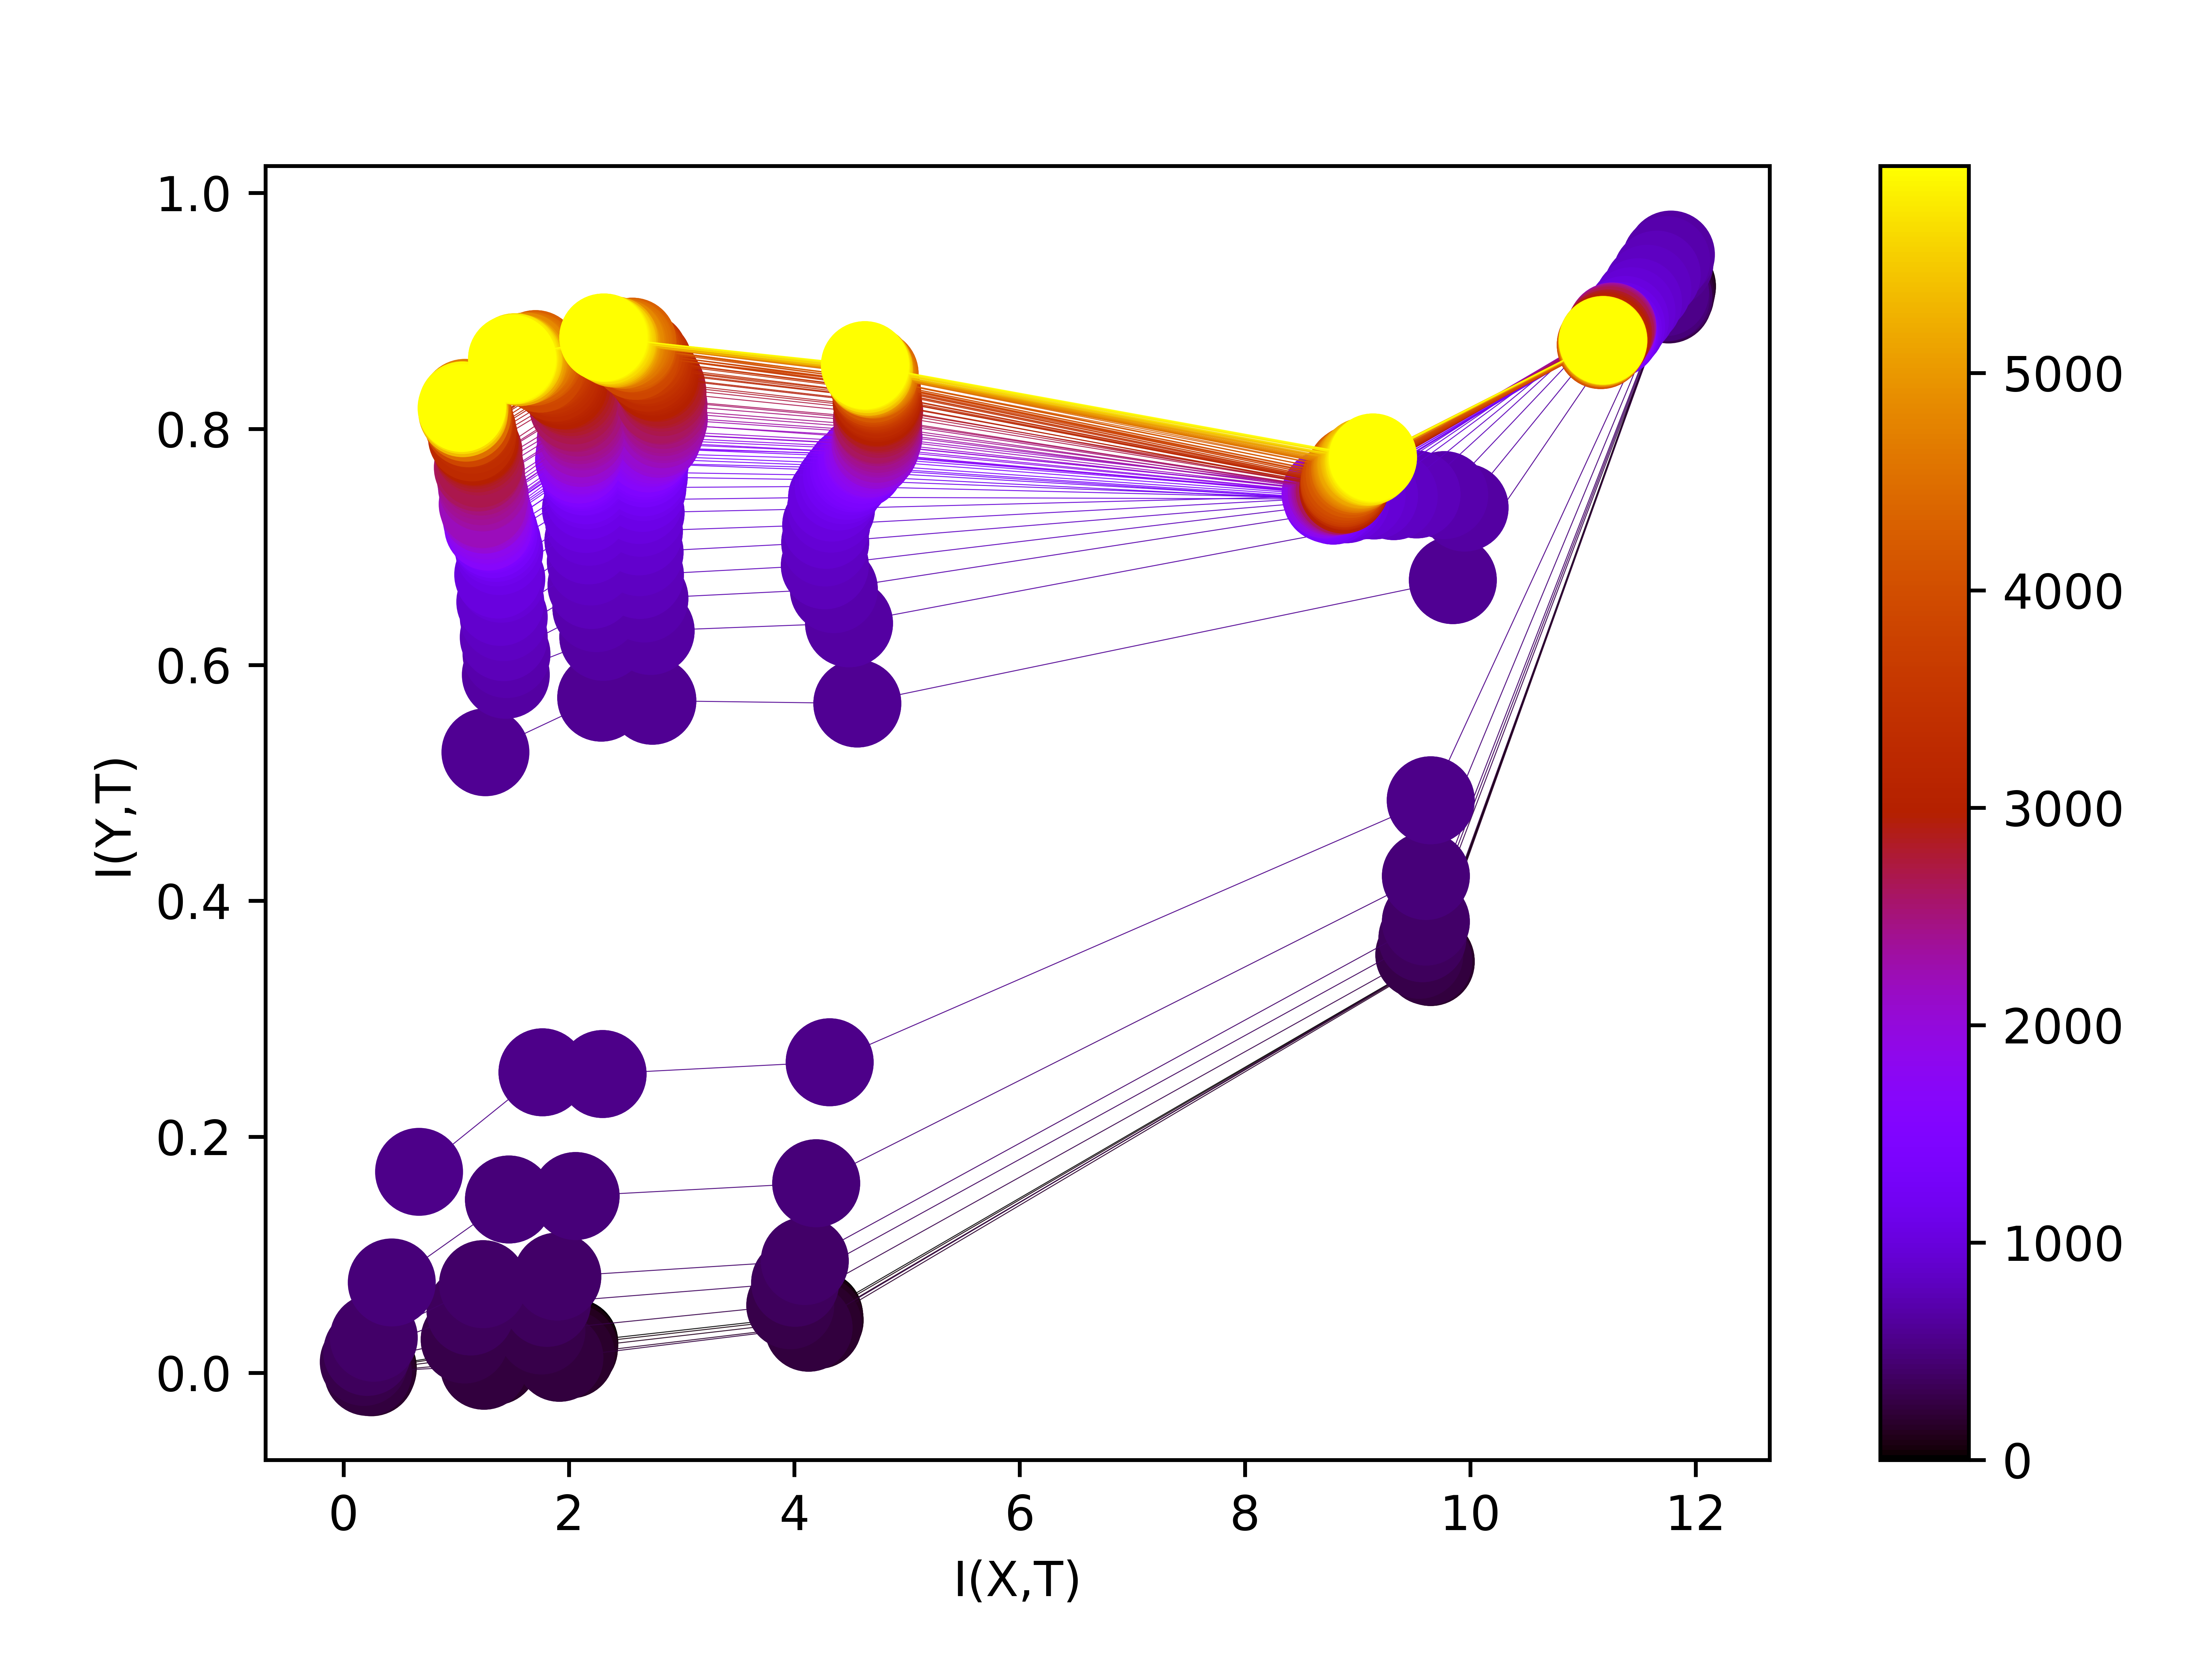
\includegraphics[width=\textwidth]{figs/eval/networkShape/KDE10,4,2,2.png}
    \caption{
      Network Shape - 12,10,4,2,2,2
    }
    \label{figNetworkShapeDefault}
  \end{subfigure}
  \hfill
  \begin{subfigure}[t]{0.32\textwidth}
    \centering
    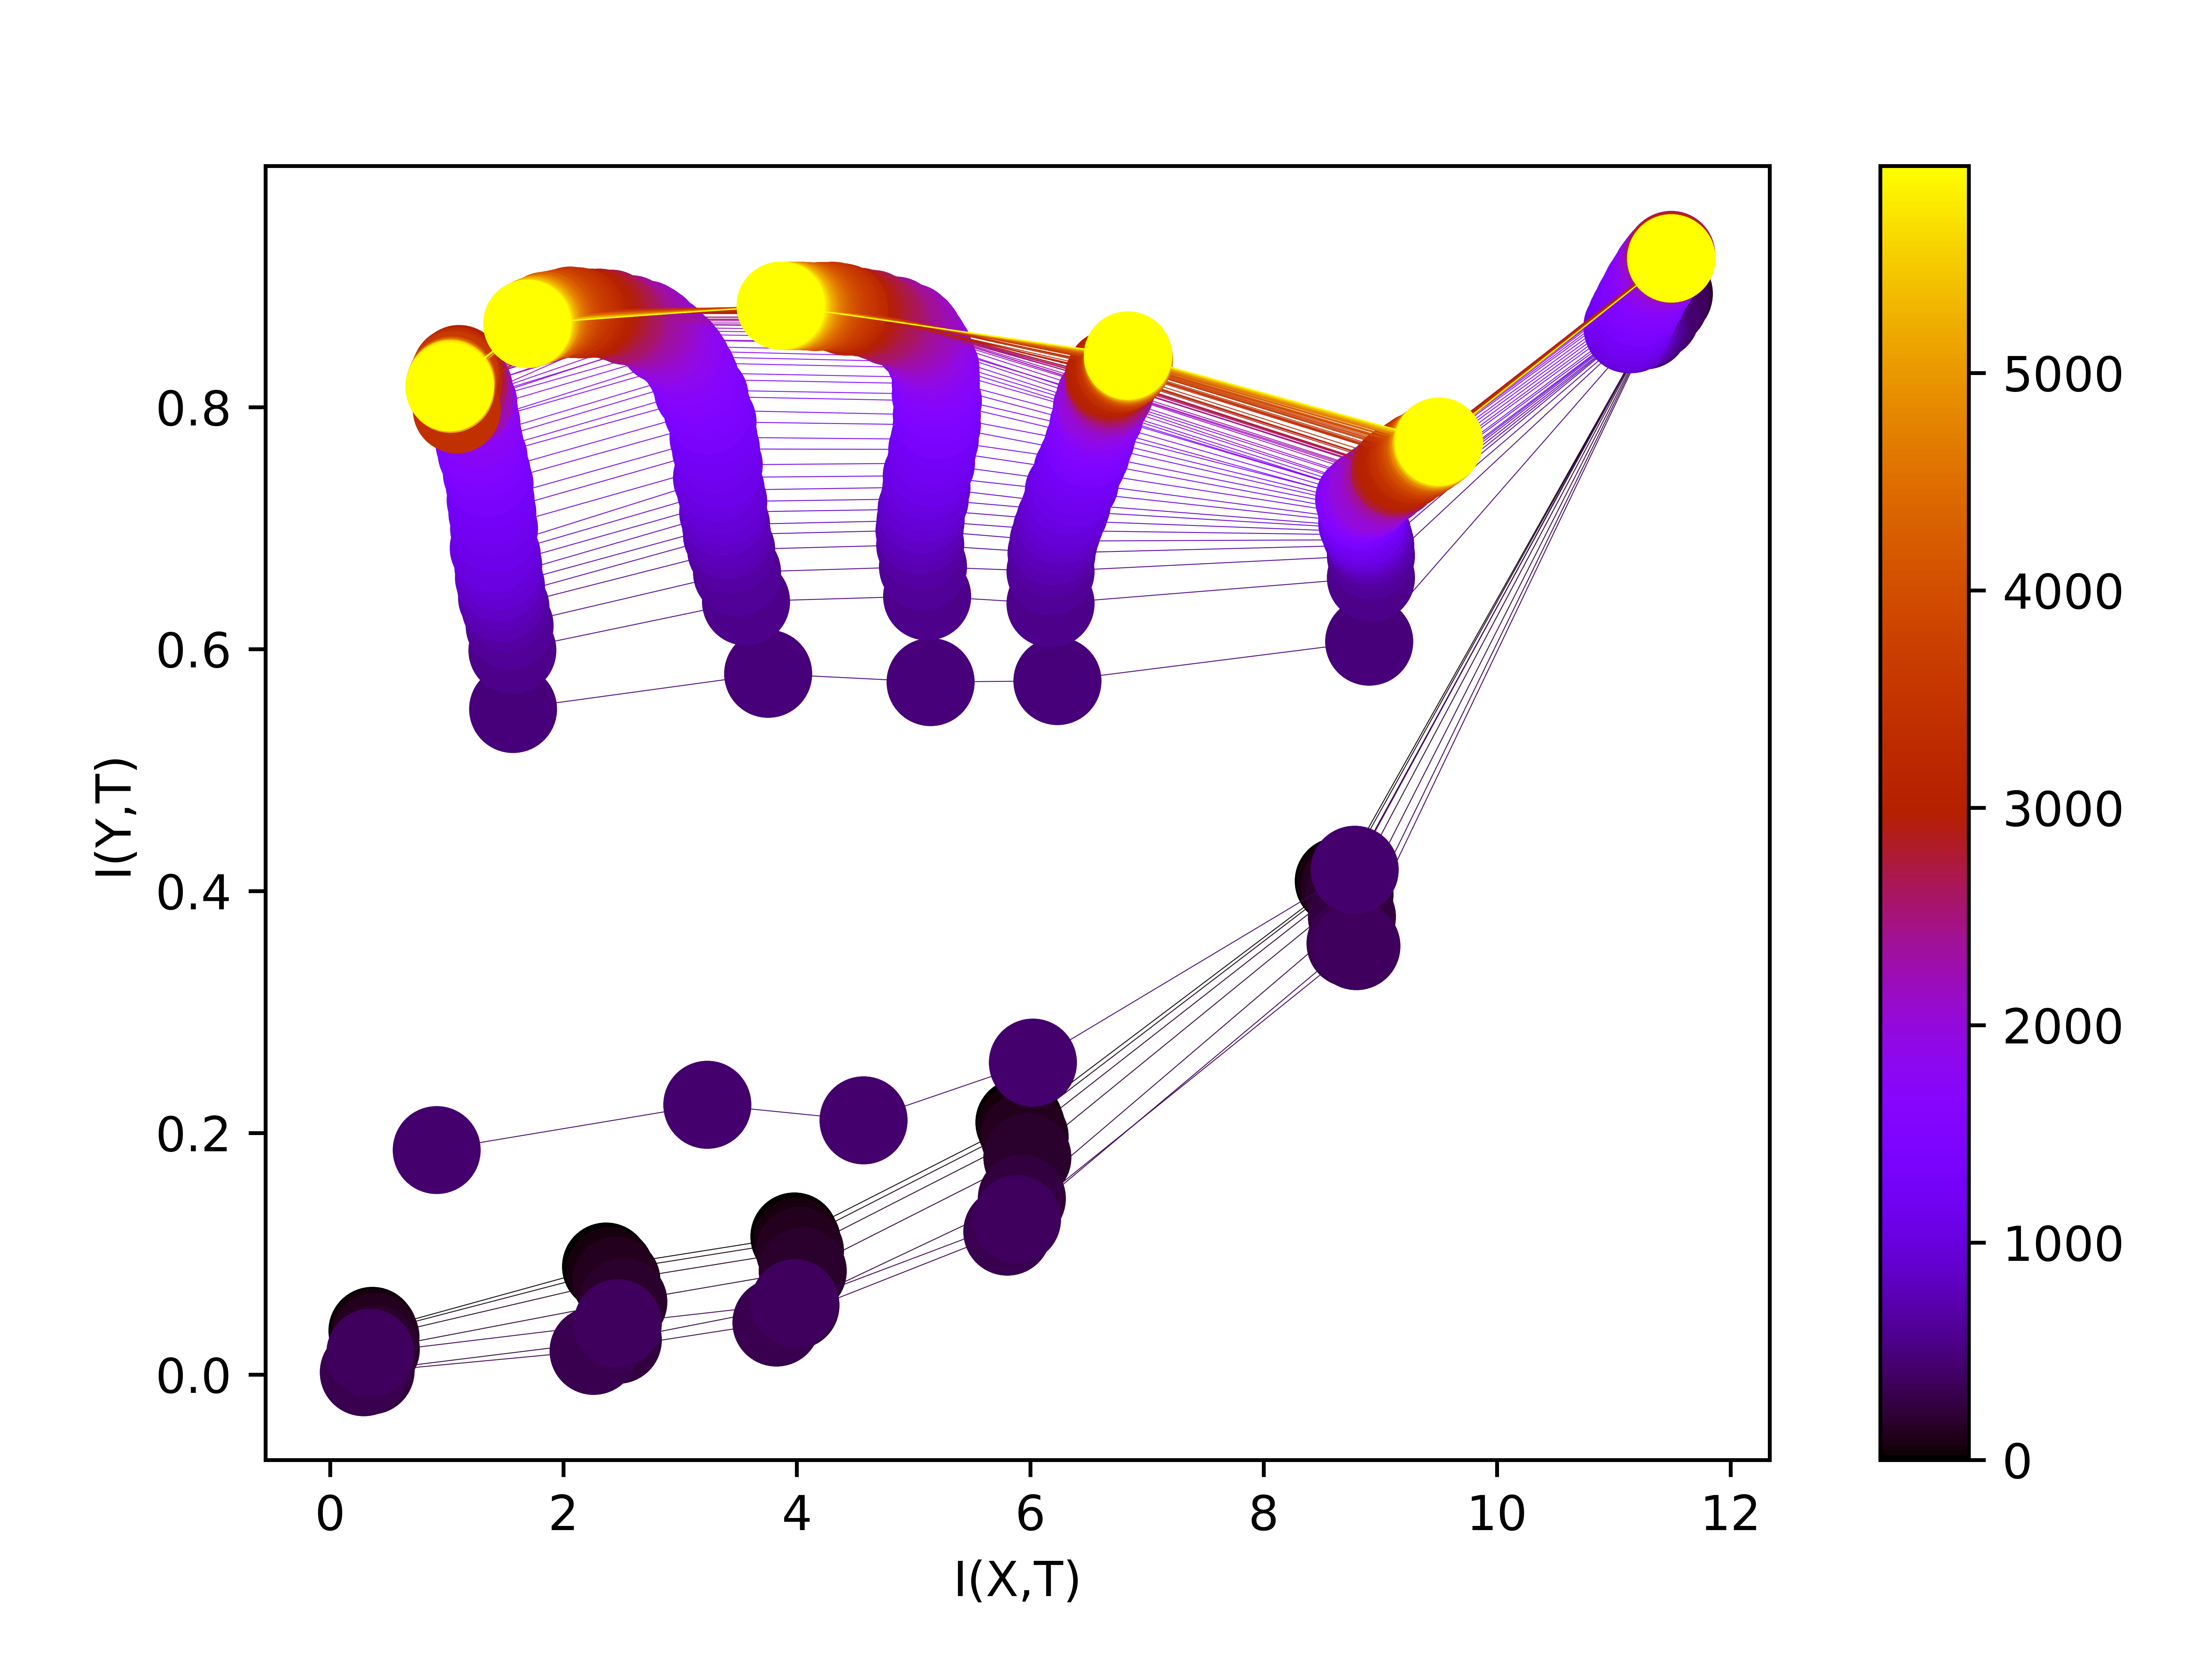
\includegraphics[width=\textwidth]{figs/eval/networkShape/KDE10,8,6,4.png}
    \caption{
      Network Shape - 12,10,8,6,4,2, Default
    }
    \label{figNetworkShape2}
  \end{subfigure}
  \hfill
  \begin{subfigure}[t]{0.32\textwidth}
    \centering
    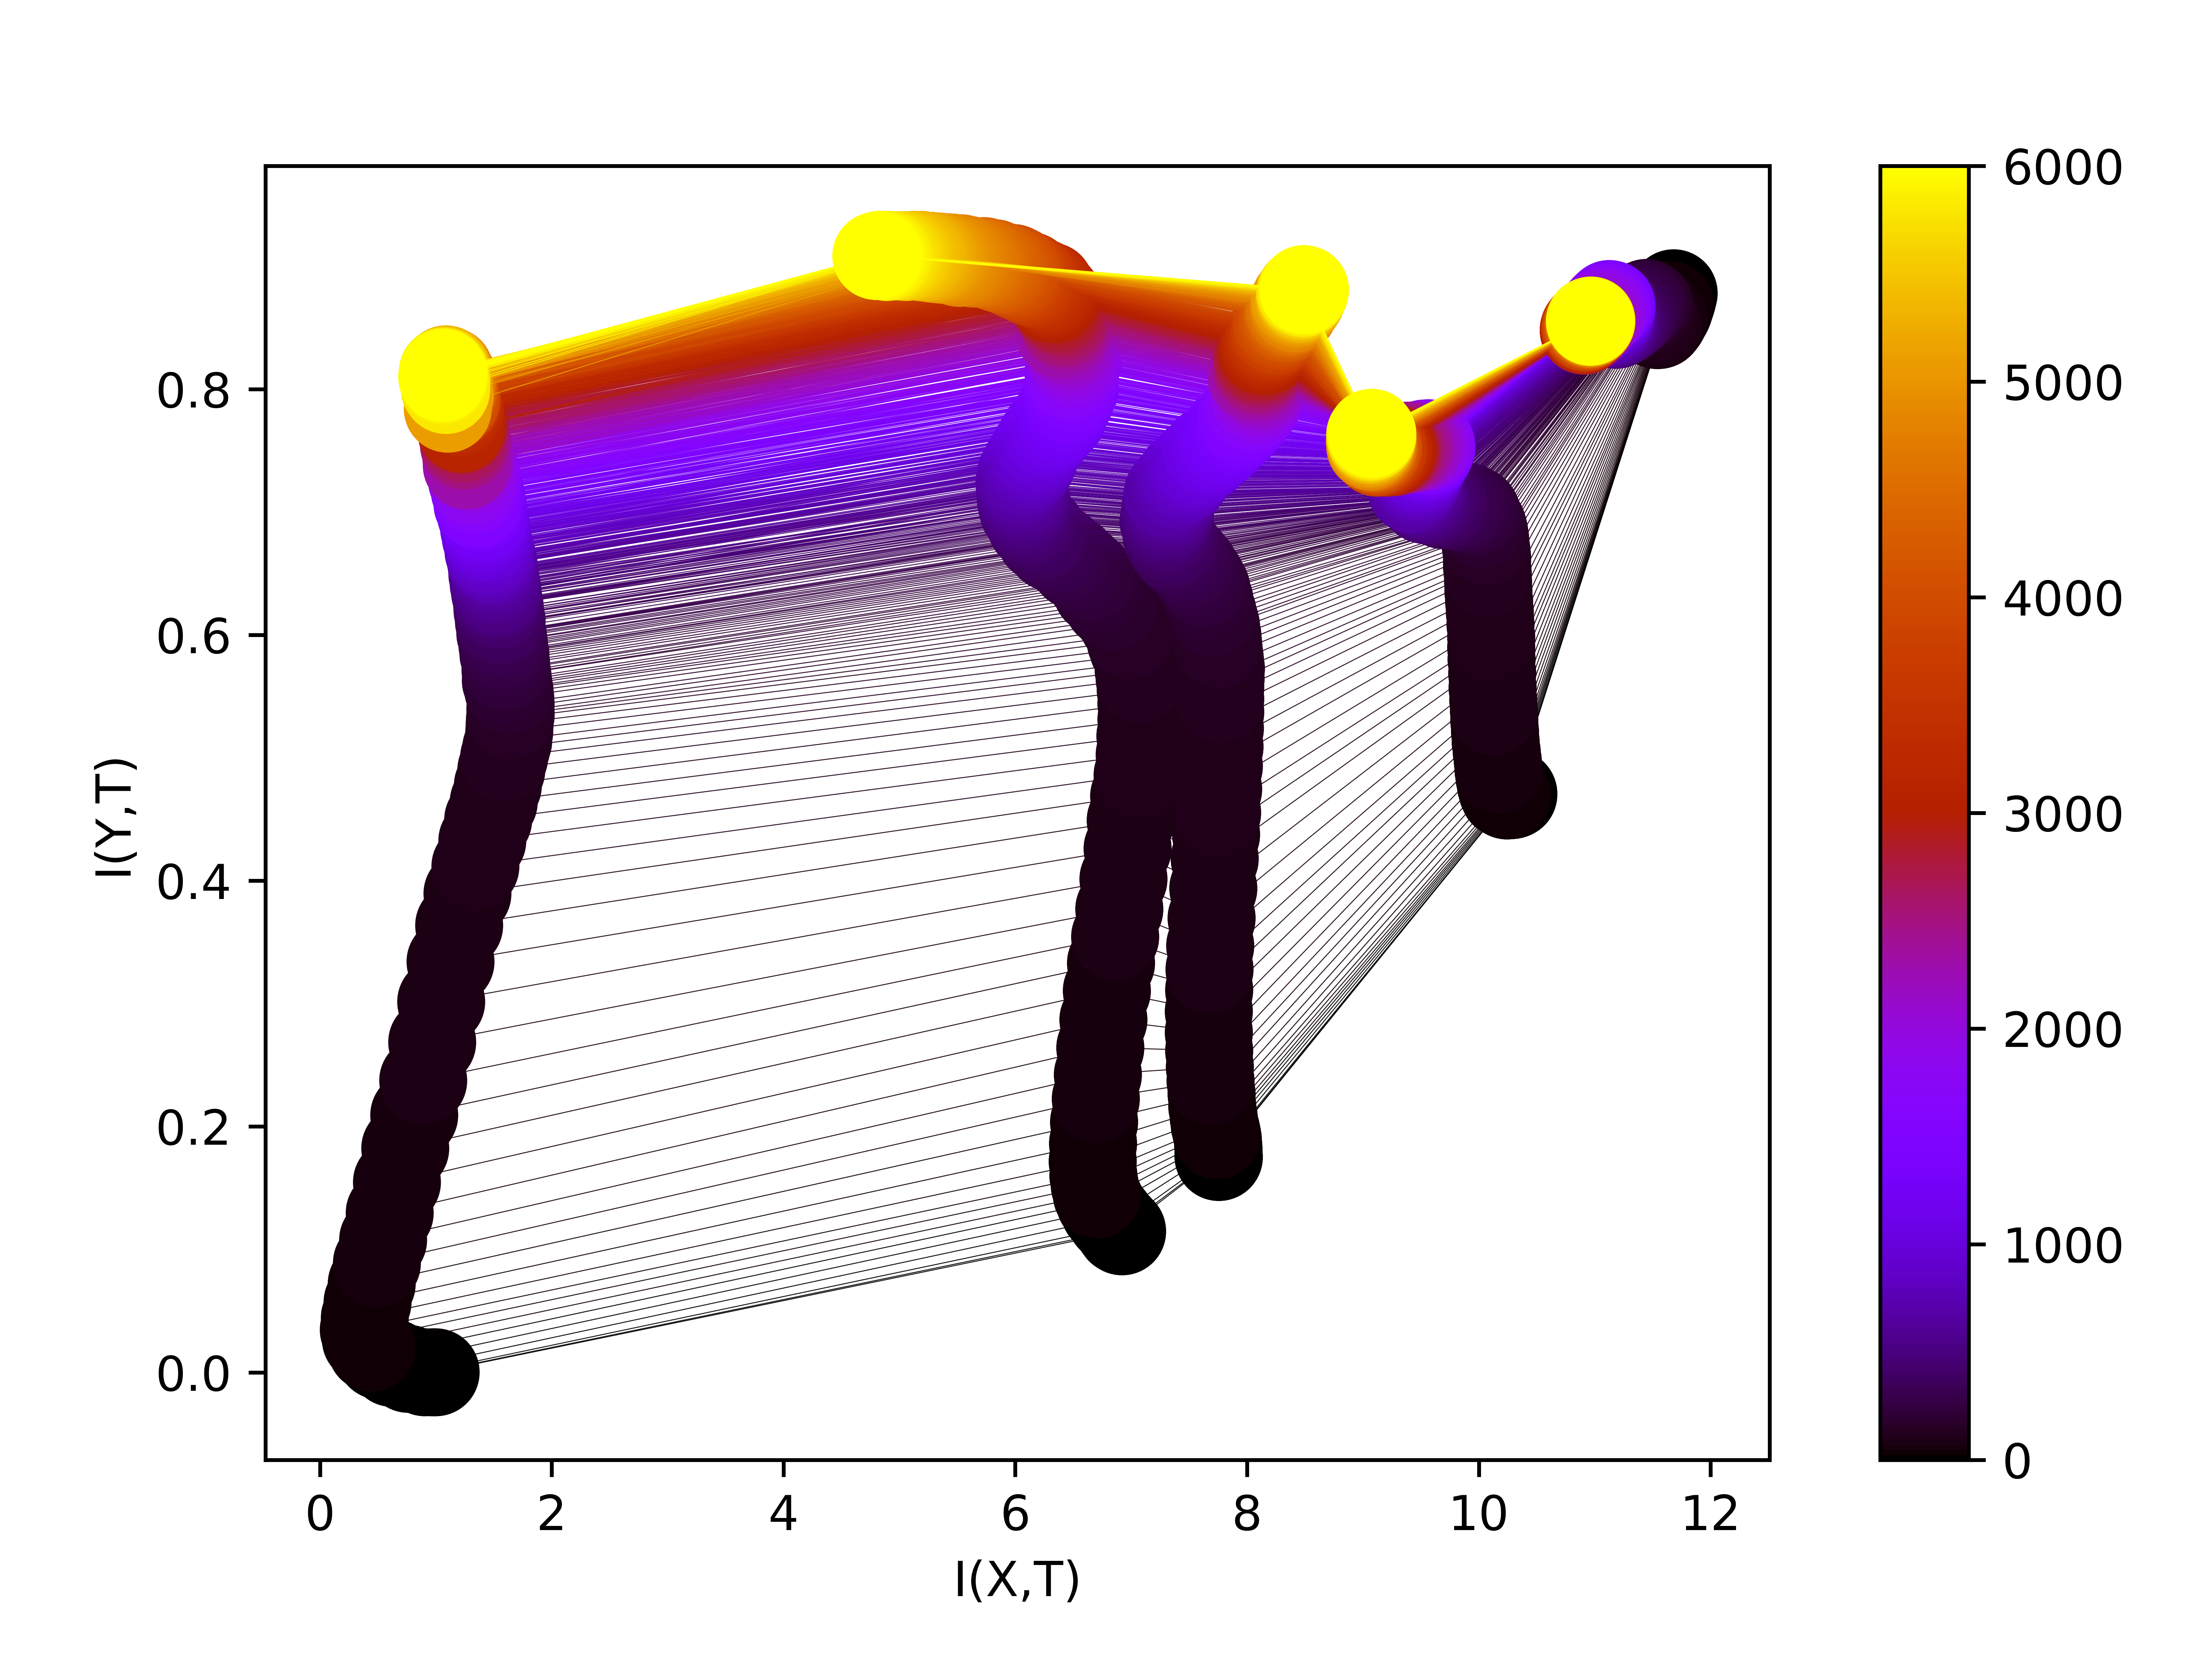
\includegraphics[width=\textwidth]{figs/eval/networkShape/KDE12,12,12.png}
    \caption{
      Network Shape - 12,12,12,12,2
    }
    \label{figNetworkShape3}
  \end{subfigure}
  \hfill
  \caption{
      $\tanh$: Demonstrating KDE for different network shapes.  Tweaking training
      size for Tishby's KDE MIE. Hyperparameters: Dataset - Tishby's, activation
      function - $\tanh$, batch size - 512, training size - 40\%.
    }
  \label{figNetworkShapes}
\end{figure}
  
\end{document}
